\documentclass[a4paper,12pt]{report}
\usepackage[utf8]{inputenc}
\usepackage{graphicx}
\usepackage{listings}
\usepackage{todonotes}
\usepackage{xcolor}
\usepackage{hyperref}
\usepackage{refcheck}
\usepackage{textcomp}
\usepackage{float}
\graphicspath{{img/}}

% draft più leggibile
\usepackage[a4paper,top=2cm,bottom=2cm,outer=5cm,verbose,headheight=1cm,heightrounded]{geometry}
\setlength{\marginparwidth}{4.5cm} %per farci stare todonotes

% copia e incolla da overleaf
\definecolor{codegreen}{rgb}{0,0.6,0}
\definecolor{codegray}{rgb}{0.5,0.5,0.5}
\definecolor{codepurple}{rgb}{0.58,0,0.82}
\definecolor{backcolour}{rgb}{0.95,0.95,0.92}
\lstdefinestyle{mystyle}{
	backgroundcolor=\color{backcolour},   
	commentstyle=\color{codegreen},
	keywordstyle=\color{magenta},
	numberstyle=\tiny\color{codegray},
	stringstyle=\color{codepurple},
	basicstyle=\ttfamily\footnotesize,
	breakatwhitespace=false,         
	breaklines=true,                 
	captionpos=b,                    
	keepspaces=true,                 
	numbers=left,                    
	numbersep=5pt,                  
	showspaces=false,                
	showstringspaces=false,
	showtabs=false,                  
	tabsize=2
}
\lstset{style=mystyle}

\begin{document}
\begin{titlepage}
	\begin{center}
		
\includegraphics[width=\textwidth]{Logo.jpg}
		\large{Corso di Laurea Triennale in Informatica}
		
		\vspace{1.8cm}
		
		\Large{\textbf{CONFRONTO TRA AUTOMOBILE E MEZZI ALTERNATIVI NEL COMUNE DI MILANO BASATO SU STIME DI TEMPI DI PERCORRENZA}}
		
		\vspace{1.8cm}
		
		\large{Tesi di Laurea di} \\
		\large{\textbf{MAURO MASTRAPASQUA}} \\
		\large{Matricola 892629}
	\end{center}

	\begin{flushleft}
		\vspace{1.8cm}
		
		\normalsize{Relatore} \\
		\normalsize{\textbf{Andrea Trentini}}

		\vspace{0.4cm}

		\normalsize{Correlatore} \\
		\normalsize{\textbf{Dario Malchiodi}}
	\end{flushleft}

	\begin{center}
		\vspace{1.8cm}
		
		\large{Anno Accademico 2020/2021}
	\end{center}
\end{titlepage}

\tableofcontents
\listoftodos

\chapter{Introduzione}
\section{Uso dell'automobile in città}

La mobilità a corto raggio è una percentuale dominante in Italia. È stato stimato che il 75\% degli spostamenti sul territorio italiano è lungo meno di 10 km, e di questi poco meno della metà sono inferiori ai 2 km\cite{isfortaudimob}. Il mezzo principale scelto per spostarsi all'interno di un'area urbana è l'auto di proprietà, che copre circa l'82\% del totale degli spostamenti. Non stupisce che da diversi anni l'Italia è il secondo Paese in Europa col maggior numero di auto per abitanti, con circa 640 auto ogni 1000 abitanti\cite{eurostatcars}, dietro solamente al Lussemburgo, con una popolazione di due ordini di grandezza inferiori alla nostra. Nell'ultimo studio annuale di TomTom del 2019\cite{tomtomindexmilan}, Milano rientra tra le prime 110 città su scala globale per livello di congestione stradale, con un traffico tale da far aumentare di quasi il 50\% il tempo impiegato a percorrere una tratta durante le ore di picco. Sono queste le principali motivazioni che hanno accelerato lo sviluppo della rete stradale e della rete ATM, l'Azienda Trasporti Milanesi, per migliorare gli spostamenti attuali e favorire la mobilità alternativa. Molti sono stati i cambiamenti apportati alla città per fronteggiare la domanda crescente di spostamenti e al contempo diminuire il traffico stradale, tra queste si citano la realizzazione della Linea M5, l'introduzione dell'area C e delle numerose zone a traffico limitato (ZTL), l'aumento delle strade a corsia preferenziale e la creazione di piste ciclabili, e infine la concessione alle aziende nel campo della mobilità condivisa.

A fronte di questi dati, viene spontaneo chiedersi quanto sia influenzato il tempo di percorrenza in auto su strade cittadine e, soprattutto, se questa influenza sia tale da favorire altri mezzi di trasporto. Sebbene sia un dato di fatto che, su strada, un'automobile sia più veloce di un tram o di una bicicletta, dall'altra bisogna ricordare dei vantaggi di cui godono gli altri mezzi. Basti pensare alle numerose strade con corsia preferenziale o carreggiata a parte per bus e tram, alle lunghe piste ciclabili che ultimamente sono state create per favorire la mobilità alternativa, fino a mezzi che non soffrono minimamente dei problemi del traffico, come le metropolitane ATM e i passanti ferroviari Trenord.

L'obbiettivo dello studio è quello di analizzare a livello di tempistiche l'impiego dell'automobile private a motore termico, che rappresentano il 99.5\% del parco auto\cite{anfiastudiestatistiche}, all'interno del Comune di Milano e confrontarlo con mezzi alternativi per gli spostamenti al suo interno, al fine di capire se l'influenza delle congestioni che caratterizzano le strade di città medio-grandi è tale da favorire i mezzi alternativi. Le principali motivazioni risiedono nel costo e nei problemi derivati dal largo impiego di tale mezzo.

\section{Problemi}

L'automobile a motore termico ha diversi problemi. Primo tra tutti è sicuramente l'\textbf{inquinamento}. I dati del 2018 dell'Automobile Club d'Italia (ACI) riportano come il 63\% delle auto in circolazione sia di categoria Euro IV o minore\cite{anfiastudiestatistiche}, dove Euro IV è uno standard sulle emissioni introdotto nel 2006 e superato nel 2008 dall'Euro V, ben 12 anni fa\cite{euroivstandard}. Nel periodo 2008-2017 compresi, l'Italia ha superato in modo continuato i limiti giornalieri e annuali di livello di polveri sottili PM10, e per questo è stata multata dalla Corte di Giustizia dell'Unione Europea a pagare una cospicua multa\cite{eunewssanzioneitalia}. Se visto in prospettiva, l'inquinamento prodotto dalle auto non è una percentuale rilevante dell'inquinamento dell'aria, difatti è emerso in numerosissimi studi effettuati in diverse città del mondo, tra cui Milano e Brescia\cite{collivignarelli2020}\cite{camaletti2020}, durante periodo locale di lockdown per l'emergenza da COVID19, che, anche a fronte di un traffico pressochè nullo, nell'aria si sono registrati gli stessi livelli di sostanze chimiche dannose registrati nei periodi precedenti in condizioni di traffico abituale, con lievi abbassamenti riguardanti le sostanze riconducibili direttamente alla combustione dei motori termici. Questi studi infatti suggeriscono che la maggior parte dell'inquinamento dell'aria è legata a fattori ambientali. Una conclusione simile è stata ottenuta analizzando i dati dell'inquinamento dell'aria nelle aree dove è stata introdotta una restrizione sulla circolazione di alcuni veicoli, come l'area C nel Comune di Milano (ex Ecopass), che concretamente ha dato scarsi risultati\cite{trentini2014}. Nonstante questo però, non bisogna dimenticare che i gas di scarico derivanti dai motori diesel risultano sicuri cancerogeni per l'uomo, al pari del fumo di tabacco, con la sottile differenza che quest'ultimo è qualcosa che si può evitare\cite{iarctable}. L'inquinamento dunque rimane un problema, dal momento che è maggiormente presente nelle città e negli agglomerati urbani, dove è presente la maggior parte della popolazione e dove le automobili, a livello di consumo di combustibile, risultano meno efficienti per via delle basse velocità.

Secondo problema dell'auto, se comparato con gli altri mezzi di trasporto per uso cittadino, è il \textbf{costo}. Una stima svolta da SosTariffe nel 2019 mostra come mantenere un'auto in Italia costi circa €1,620 all'anno, compresi di assicurazione, benzina e bollo auto, esclusi il prezzo del mezzo stesso, che si aggira intorno ai €11,000 per un'utilitaria a chilometro zero, il cambio delle gomme ed eventuali imprevisti\cite{sostariffe}. Seppur questo problema risulti molto relativo, dato che è il reddito e il patrimonio di una persona a incidere sulla percezione di questa spesa, il solo costo di mantenimento di un'auto risulta molto più dispendioso rispetto ai mezzi alternativi, come un abbonamento annuale per i mezzi pubblici, per treni, o come l'acquisto e il mantenimento di una bicicletta o di mezzi alternativi.

Ultimo ma non ultimo dei problemi è l'\textbf{efficienza} dell'auto in termini di tempo all'interno delle grandi città, come già citato precedentemente. Tra le proprietà che caratterizzano lo spostamento in auto vi è sicuramente l'ingombro stradale rapportato al numero di persone in viaggio, ovvero l'utilizzo dell'automobile per lo spostamento del solo conducente, nonostante la capacità maggiore dell'auto, che congestiona le strade per un flusso di persone relativamente minore di persone rispetto a un bus. A documentarlo è l'Associazione Nazionale Comuni Italiani (ANCI), che ha stimato che, degli 1.8 milioni di veicoli che si spostano quotidianamente nelle città italiane per tragitti casa-lavoro o casa-studio, 1.2 milioni viaggiano con solo il conducente a bordo\cite{anciperrepubblica}, più del 66\%.

\section{Vantaggi}

A giustificare la grande diffusione di questo mezzo di trasporto tra la popolazione sono sicuramente i grandi vantaggi che l'uso o il possesso di un auto comportano. Prima di tutto, possedere un auto può essere considerato sinonimo di libertà di muoversi: non si hanno limiti di orario di partenza, perchè l'auto è pronta per essere usata a qualsiasi ora. La decisione dell'orario di inizio viaggio è esclusivamente del conducente, al contrario dei mezzi pubblici dove l'orario di partenza è offerto in numero limitato e prestabilito, con scarse percorrenze negli orari notturni; non si hanno limiti di distanza, perchè in automobile si può percorrere qualsiasi distanza senza particolari sforzi fisici, al contrario della bicicletta; non si hanno limiti di destinazione, perchè essenzialmente con l'automobile si può raggiungere qualsiasi posto raggiungibile con i mezzi alternativi e non; si possono trasportare merci molto pesanti, difatti uno tra gli impieghi principali dell'auto, dopo quello del raggiungimento del luogo di lavoro e/o di studio, è quello di fare la spesa al supermercato e quello legato al trasporto di merce ingombrante acquistata, difficile da trasportare in assenza di un veicolo e spesso delegata a chi fornisce servizi di spedizioni. Altri vantaggi legati all'auto sono legati alla sua comodità e praticità. Per esempio, nel Comune di Milano, la maggioranza dei parcheggi sono riservati ai residenti e sono divisi a zone, garantendo la possibilità di trovare parcheggio nei pressi della propria abitazione, sebbene tale provvedimento sia stato pensato originariamente a ostacolare gli spostamenti in auto all'interno della città. Inoltre, in caso di pioggia, temporale e persino neve, viaggiare in auto risulta l'opzione più comoda e sicura, talvolta l'unica funzionante.

\section{Confronto con mezzi alternativi}

È sul terzo problema che si concentra questo studio, che ha come obbiettivo capire quanto sia vantaggioso o svantaggioso in termini di tempi di percorrenza usare un'automobile all'interno della città di Milano, a fronte di problemi come traffico e congestioni stradali, da parte di una persona con pure esigenze di spostamento, senza vincoli legati a trasporto merci, intemperie o raggiungimento di luoghi al di fuori della città. Per capire quale sia il mezzo più vantaggioso, la soluzione ideale sarebbe quella di organizzare diverse gare in diversi punti della città, in cui delle persone, ognuno con un mezzo di trasporto diverso, partono da un comune punto di partenza e raggiungono un comune punto di destinazione, cronometrando il tempo impiegato da ciascuno. Purtroppo, non avendo a disposizione le risorse e il tempo (e, date le restrizioni per la pandemia di COVID19, nemmeno il permesso) per effettuare un confronto del genere, si è optato per una soluzione informatica.


\chapter{Metodi}
L'idea alla base di questo studio è, dunque, quella di confrontare diversi mezzi di trasporto su percorsi comuni, ovvero con punto di partenza, di destinazione, di data e orario di partenza uguali, salvando il tempo impiegato da ciascun mezzo per compiere il tragitto e usare successivamente tali valori per effettuare delle analisi, con l'obbiettivo finale di dichiarare un vincitore e, specialmente, capire di quanto abbia vinto. Infatti, non ci si aspetta un risultato diverso da quello che vede l'automobile come vincitore, ma si vuole analizzare se questo vantaggio sia relativamente grande dal punto di vista di una persona e se esistano delle variazioni lungo l'arco della giornata di questo vantaggio, visti i problemi relativi al traffico e di congestione stradale di cui le grandi città soffrono. Avendo a disposizione i dati relativi al percorso di confronto e al tempo impiegato dai vari mezzi, si possono effettuare ulteriori analisi, come le prestazioni di ogni mezzo in termini di velocità media, la variazione di ora in ora di quest'ultima o per esempio l'influenza che ha la lunghezza della tratta sulla velocità media.

Purtroppo però, un dataset contenente i tempi di percorrenza di tragitti comuni effettuati da diversi utenti su diversi mezzi di trasporto non esiste, molto probabilmente perchè nessuno l'ha mai veramente effettuato un confronto del genere. Gli unici che possiedono un dataset del genere di tratte realmente effettuate ma con un singolo mezzo sono le aziende private che offrono il servizio di navigazione, come per esempio Google Maps, Waze, Moovit, TomTom. Tali aziende infatti offrono applicazioni per poter guidare l'utente da un punto A ad un punto B con un determinato mezzo, per esempio mezzi pubblici, in tempo reale e col tracking GPS, e dato che il servizio nella maggior parte delle volte è offerto gratis, il pagamento per il servizio è effettuato coi dati del viaggio effettuato, e non hanno alcun incentivo nel pubblicare, anche in sola parte, i dati che hanno raccolto, nonostante siano i loro utenti i veri proprietari dei dati generati.

\section{Open Data}

La pubblicazione totale o parziale di questi dati è una pratica ancora poco diffusa che rientra nella filosofia dell'\emph{Open Data}. Secondo questa filosofia, simile a quella dell'\emph{open-source}, i dati dovrebbero essere liberamente accessibili da chiunque, senza nessun tipo di restrizioni derivanti da \emph{copyright}, patentini o altri meccanismi di controllo che riguarda la loro ridistribuzione. Uno dei campi che maggiormente beneficerebbe di questa filosofia sarebbe proprio la ricerca scientifica, che grazie all'accesso facilitato a questi dati riuscirebbe ad accelerare i tempi delle scoperte, e di conseguenza perfino le aziende stesse che possiedono questi dati ne gioverebbero. Non a caso sono già molti gli studi effettuati basati su dati acquisiti tramite scraping di siti web che sono riusciti a dare un contributo sia in ambito di ricerca e sia all'azienda stessa. Di questi vi è una sottocategoria dedicata ai trasporti. In questa categoria, un tema di spicco tra tutti è l'analisi dei dati prodotti dai servizi di mobilità condivisa. In uno studio effettuato a Milano nel 2014\cite{croci2014} sul bike sharing di ATM chiamato BikeMi, si è scoperto che nelle vicinanze di stazioni ferroviarie e università in zone di circolazione ristretta, il servizio veniva maggiormente usato rispetto ad altri posti. Un altro studio del 2017 effettuato sempre a Milano \cite{pagani2017} propone un sistema di nome Knowledge Discovery System basato su dati di 3 servizi di car sharing, Car2Go, Enjoy e Twist, in grado di offrire stime in tempo reale del percorso e di rilevare le zone in cui la richiesta del servizio è alta e le auto a disposizione scarseggiano. In questo studio inoltre viene evidenziato che durante il giorno le auto sono maggiormente concrentrate nella zona centrale di Milano mentre durante la sera si riversano nelle zone suburbane. In entrambi i due studi presi come esempio sono emerse delle informazioni che risulterebbero molto preziose per le aziende fornitrici dei servizi e che, di conseguenza, se venissero prese in considerazione, aumenterebbe lo sfruttamento del servizio da parte degli utenti.

Nonostance ciò, pochissime se non nessuna delle aziende che possiede dati generati dagli utenti ha mai reso disponibile apertamente quello che ha raccolto. Alcune di esse, come TomTom, si limitano a pubblicare regolarmente delle infografiche statistiche basate sui dati in loro possesso. Altre ancora si limitano a usare tali dati per autopromuoversi online e quindi farsi pubblicità. Queste pratiche però risultano problematiche sotto diversi aspetti, primo tra tutti è l'impossibilità di verificare le informazioni trasmesse, dato che la sorgente è nascosta, risultando quindi poco credibili considerando l'interesse primario di un'azienda in ambito economico. Un secondo problema, dal punto di vista dell'azienda, è quello di dover schierare, e quindi pagare, analisti di dati per produrre tali statistiche che però non hanno alcuna valenza scientifica, quando potrebbero solamente incaricarsi di rendere anonimi dei dati e pubblicarli, per ricevere gratuitamente studi fatti su tali dati da studenti e ricercatori di tutte le parti del mondo e che hanno una valenza scientifica.

\section{Prototipi}

Avendo l'accesso allo storico dei viaggi effettuati dagli utenti di più servizi, ognuno legato a un mezzo di trasporto, come Moovit per i mezzi pubblici e Waze per l'automobile, si potrebbero cercare delle tratte simili nei dataset di ognuno di essi, ovvero percorsi di viaggiatori che inconsapevolmente hanno condiviso punto di partenza e punto di arrivo, per confrontare i tempi di percorrenza. Tenendo conto che sarebbe poco efficiace usare un operatore di uguaglianza su delle coordinate geografiche prodotte da viaggiatori, dato che risulterebbero poche quelle che effettivamente coincidono, il che vorrebbe dire persone diverse che hanno fatto lo stesso identico viaggio, il modo migliore per catturare dei tragitti comuni sarebbe quello di considerare tali coordinate di partenza e di arrivo a gruppi, ovvero circoscritti entro un certo raggio e quindi considerabili come lo stesso viaggio. Per catturare questo concetto di gruppi si potrebbe utilizzare uno degli algoritmi di clusterizzazione, che sono stati creati apposta per questo tipo di problemi. Un possibile approccio infatti sarebbe quello di fondere i dataset dei diversi servizi in un unico dataset e clusterizzare i punti di partenza e di destinazione più frequenti usando l'algoritmo di clusterizzazione DBSCAN\cite{ester1996} o una delle sue varianti ottimizzate appositamente per dati geospaziali\cite{zhou2003}\cite{borah2004}, per mettere a confronto i mezzi di trasporto usando i viaggi appartenenti allo stesso cluster sia di partenza che di destinazione. Un approccio del genere però risulterebbe problematico sotto alcuni aspetti, primo tra tutti l'esecuzione dell'algoritmo stesso, infatti il DBSCAN ha una complessità temporale di $O(n^{2})$ e una complessità spaziale di $O(n)$ nel peggiore dei casi, complessità spaziale che arriva a $O(n^2)$ se si usa una matrice $n \times n$ per evitare delle ricomputazioni già effettuate. Per esempio, usando un campione di 100,000 viaggi, ognuno di essi contenente 2 variabili di tipo float32, e quindi di 4 Byte ciascuno, per le sole coordinate di partenza, eseguire tale algoritmo in tempi fattibili, e quindi utilizzando una tabella per le ricomputazioni, richiederebbe $100000^{2} \times (2 \times 4 B) = 80 GB$ di memoria centrale, il che avrebbe richiesto il noleggio di un server per tale calcolo. Un altro problema legato a questo modo di procedere, indipendentemente dall'algoritmo usato per raggruppare le tratte, è quello di trovare dei viaggi percorsi nella stessa data e allo stesso orario, che ristringerebbe il campione dei viaggi drasticamente. Difatti avrebbe poco senso confrontare viaggi eseguiti in diversi giorni e/o a orari diversi per via del traffico che caratterizza una città, nello specifico quella di Milano. Secondo diversi servizi di monitoraggio del traffico infatti, un viaggio in auto in una settimana lavorativa il lunedì mattina alle 9:00 è molto sfavorito per via del picco di congestione stradale che caratterizza quel giorno, di conseguenza, confrontarlo con un qualsiasi altro viaggio che non abbia sofferto di questo rallentamento sarebbe poco significativo. Quello che si potrebbe fare avendo a disposizione un dataset di viaggi effettuati e che risulterebbe interessante sarebbe l'analisi delle performance di ogni mezzo preso singolarmente, misurandone diversi parametri, come velocità media, e rapportare quest'ultime analisi alle condizioni storiche del traffico per misurare l'impatto di queste condizioni sulle performance.

Non avendo nemmeno quest'ultima possibilità di avere accesso a dataset di viaggi compiuti con diversi mezzi e visti i problemi che avrebbe introdotto tale approccio, si è scelto di creare un dataset di gare tra mezzi attraverso una simulazione.

\section{La simulazione}

Quado si effettua una richiesta a un servizio come Google Maps per un tragitto, quello che fa Google è calcolare, sulla base di dati in tempo reale del traffico, degli incidenti, degli orari di servizio dei mezzi pubblici e la loro posizione, una stima del tempo di percorrenza per diversi mezzi, come automobile, mezzi pubblici, tragitto a piedi e bicicletta (solo in presenza di piste ciclabili), per compiere tale tragitto. Sebbene siano solo stime e non cronometraggi realmente effettuati, esse risultano estremamente precise o quanto di più simile alla realtà. Lo stato attuale della tecnologia e la loro vasta e affermata presenza nella vita quotidiana delle persone infatti permette a tali servizi di avere informazioni sempre più precise, utilizzando tecniche come quella del crowdsourcing di dati dagli smartphone degli utilizzatori e sfruttando lo storico dei viaggi effettuati. 

\subsection{Un caso di studio: Waze}

Per fare un esempio, Waze, per fornire una stima del tempo di arrivo (in inglese nota come ETA: Estimated Time of Arrival), per prima cosa guarda i dati storici della velocità media di ogni segmento di strada compreso nell'itinerario calcolato. Questo particolare dato viene aggiornato ogni 30 minuti usando i dati prodotti dallo smartphone dei loro utenti, e nel caso non sia presente nessun dato la ricerca procede a ritroso fino alle ultime 8 settimane. In secondo luogo usa i dati in tempo reale che ha a disposizione degli utenti connessi e dei dati del traffico. Infine, tramite filtri per eliminare gli outlier, ovvero gli utenti estremamente veloci o lenti, ed equazioni matematiche danno una stima del tempo di percorrenza. Inoltre, tale stima viene aggiornata in tempo reale man mano che si procede nel viaggio, sempre tramite i dati collezionati da altri utenti. Quello che infatti ci tiene a sottolineare Waze e che la rende competitiva è la stima dei tempi di percorrenza basata interamente sulla loro community di utenti, dove ogni singola persona che usa la loro app contribuisce al bene di tutti migliorando le stime successive\cite{wazeblog}.


\chapter{Progettazione}
Per attuare questo confronto tra mezzi di trasporto si è scelto di appoggiarsi a servizi di navigazione in grado di fornire stime di percorrenza (Estimated time of arrival, ETA) in tempo reale e usarle come valori effettivi. Le gare per confrontare tali mezzi sono state tradotte in richieste di stime di percorrenza per un tragitto comune a tutti, effettuate più volte al giorno e per diversi percorsi. In questo modo si riuscirebbe nell'intento iniziale di effettuare uno studio su degli stessi percorsi iniziati nello stesso momento ma con mezzi di trasporto diversi. Sono stati presi in considerazione i principali mezzi di trasporto alternativi all'automobile di proprietà con cui è possibile spostarsi all'interno del Comune di Milano:
\begin{itemize}
	\item automobile;
	\item servizio di car sharing Enjoy;
	\item mezzi pubblici ATM e passanti ferroviari Trenord;
	\item bicicletta;
	\item a piedi.
\end{itemize}
Quest'ultimo, anche se non diretto competitor, è stato scelto per essere usato come riferimento.

\section{Ricerca delle API}

Il primo passo verso la scrittura di un software per effettuare le varie richieste di percorso è stata quella di cercare delle API disponibili per ogni mezzo di trasporto in grado di fornire stime dinamiche sui tempi di percorrenza basate su dati in tempo reale.

\subsection{Google (auto, bici e a piedi)}

Inevitabilmente Google è stata la prima opzione che si è cercata. Google infatti, grazie a Maps e grazie all'acquisizione di Waze\cite{googleblog}, è una dei leader nel settore delle informazioni di navigazione e che vende la loro conoscenza tramite API. Tra le varie API offerte è presente quella che fa il caso di questo studio, la Directions API, che è in grado di fornire stime di percorrenza molto precise per l'auto, per il percorso a piedi e per la bicicletta (quando disponibile)\cite{googleapi}. Purtroppo però, il costo per l'utilizzo di queste API è di 10\$ per 1000 richieste al mese, l'equivalente di circa 1 richiesta all'ora, che risulta troppo poco per l'obbiettivo dello studio di catturare la variazione delle performance dei mezzi di ora in ora\cite{googleapiprice}.

\subsection{Waze (auto)}

Nonostante sia stata acquisita da Google, Waze è rimasta indipendente a livello di API. Quello che offre Waze però non è esattamente un endpoint a cui fare richiesta per un determinato viaggio, ma semplicemente degli URL da inserire nel proprio sito web o nella propria app Android/iOs per aprire il client Waze da browser/app coi dati della richiesta parametrizzati nell'URL\cite{wazeapi}.

\subsection{Moovit (mezzi pubblici)}

Anche Moovit non offre API per interrogare direttamente i loro servizi e ricevere delle stime, ma solamente l'opzione di incorporare un widget all'iterno della propria pagina web o applicazione che rimanda direttamente ai loro servizi\cite{moovitapi}.

\subsection{Here (auto, scooter e mezzi pubblici)}

Il servizio Here offre una REST API per le informazioni riguardo il routing e la stima del tempo di percorrenza. Queste stime però risultano accurate (basate su dati in tempo reale) solo per determinate città, comunicate sul loro sito, e tra queste non è inclusa Milano. Per le città non in lista, la stima è fatta sulla base dei dati tabellari degli orari dei passaggi dei mezzi\cite{hereapi}.

\subsection{Car2Go, Enjoy (car sharing)}

Non sono stati trovati servizi relativi a stime di tempi di percorrenza utilizzando un mezzo dei servizi car sharing. I servizi di car sharing Car2Go ed Enjoy non offrono API per tale calcolo ma dispongono di una mappa costantemente aggiornata sul loro sito web con l'elenco delle auto libere, ognuna con allegato dati riguardo il tipo di veicolo (tra auto e moto) e il carburante rimasto. Un programma in grado di acquisire le informazioni delle auto libere è stato gentilmente offerto da Federico Losacco, che lo ha scritto e utilizzato per uno studio sul comportamento del traffico basato sui viaggi compiuti dagli utenti del servizio\cite{losaccofederico}.

\subsection{OpenStreetMap e dintorni (auto, bici e a piedi)}

Il progetto collaborativo di OpenStreetMap offre, tra le altre cose, il calcolo di un tragitto usando come backend servizi offerti da terze parti, tra cui Open Source Routing Machine (OSRM). Purtroppo però, tali servizi non usano dati in tempo reale per la stima del tempo di percorrenza\cite{osm}.

\section{Scelta delle API}

Di seguito sono elencate le scelte fatte per i servizi e i loro rispettivi ruoli di copertura dei mezzi di trasporto:

\begin{itemize}
	\item HERE REST API\cite{herewegoapi}
	\begin{itemize}
		\item mezzi pubblici ATM e passanti ferroviari Trenord;
	\end{itemize}

	\item OpenStreetMap con OSRM\cite{openstreetmap}
	\begin{itemize}
		\item bicicletta e a piedi;
	\end{itemize}

	\item Enjoy Map scraper di Federico Losacco\cite{enjoycarsharing}\cite{losaccofederico}
	\begin{itemize}
		\item servizio di car sharing Enjoy;
	\end{itemize}
\end{itemize}
Nonostante OSRM non offra soluzioni in tempo reale ma statiche, è stato scelto ugualmente per via della scarsa influenza del traffico sui tempi di pecorrenza in bicicletta e a piedi, che dipendono per la maggior parte dall'itinerario calcolato e dalle caratteristiche delle strade come i segnali stradali (divieti, contromano, aree pedonali etc...).

Le API REST di Here sono state utilizzate per mancanza di valide alternative. In un primo momento si è tentato lo scraping del sito web di Moovit per interagire col sito e comunicare le richieste senza intervento umano, ma la difficoltà nel codificare i parametri delle richieste e a decodificarne le poche risposte immerse in svariati messaggi di errore ne hanno scoraggiato l'utilizzo.

Per il servizio di car sharing, si è scelto di usare la lista delle macchine libere come base, ottenuta tramite scraping, per ottenere una stima del tempo di percorrenza basata su due percorsi, per primo il tragitto a piedi per raggiungere l'auto libera più vicina al punto di partenza richiesto e come secondo il tragitto in auto per completare il percorso dal punto in cui si trova l'auto alla destinazione richiesta.

Non sono state trovate valide alternative per il servizio di routing in auto. Google risulta essere eccessivamente costosa se si considera un minimo di 10 richieste all'ora per avere un campione rappresentativo di quel giorno di diversi punti della città. Il prezzo per una prestazione del genere è di circa 72\$ al mese. Waze invece non offre nessuna API per essere interrogata direttamente. Per ovviare a questo problema, si è scelto di programmare un browser headless in grado di interagire direttamente col sito web di Waze per interrogare il servizio e prelevare i dati della stima di percorrenza, simulando per intero l'interazione umana con la pagina.

Le API REST di HERE e quelle di OpenStreetMap sono nella seguente forma:
\begin{lstlisting}[language=Go]
func stimaTragitto(a, b coordinate) durata
\end{lstlisting}
ovvero chiedono in input le coordinate di partenza e di destinazione e restituiscono in output una stima di percorrenza del tragitto in formato JSON di quel determinato momento.

\subsection{Lo scraping di Waze}

Dato che i servizi per sviluppatori offerti da Waze sono gratuiti, si è scelto di sfruttare tali dati ma prendendoli per vie laterali, direttamente dalla pagina web \url{https://www.waze.com/live-map}. La maggior parte dei browser in circolazione, come Mozilla Firefox, offrono oltre al browser in sè tutti gli strumenti da sviluppatore di siti web usati a scopo di debugging. Tra questi vi è la console da sviluppatore, apribile tramite una scorciatoia da tastiera \texttt{Ctrl+Shift+K}. Con questa console è possibile vedere le richieste di rete che il sito effettua in background per il suo funzionamento. Dato che si tratta di un'applicazione a singola pagina, è chiaro che per il suo funzionamento vengano effettuate delle richieste tramite JavaScript in modo asincrono direttamente ai loro server. Questa pratica prende il nome di Asynchronous JavaScript and XML (AJAX)\cite{ajaxwiki}. Guardando i comportamenti a livello di rete del sito web, mentre si svolge una richiesta per un viaggio a Waze, si presenta subito un URL che fa da endpoint per le richieste di routing, come mostrato nella figura \ref{image:1}.
\begin{figure}
	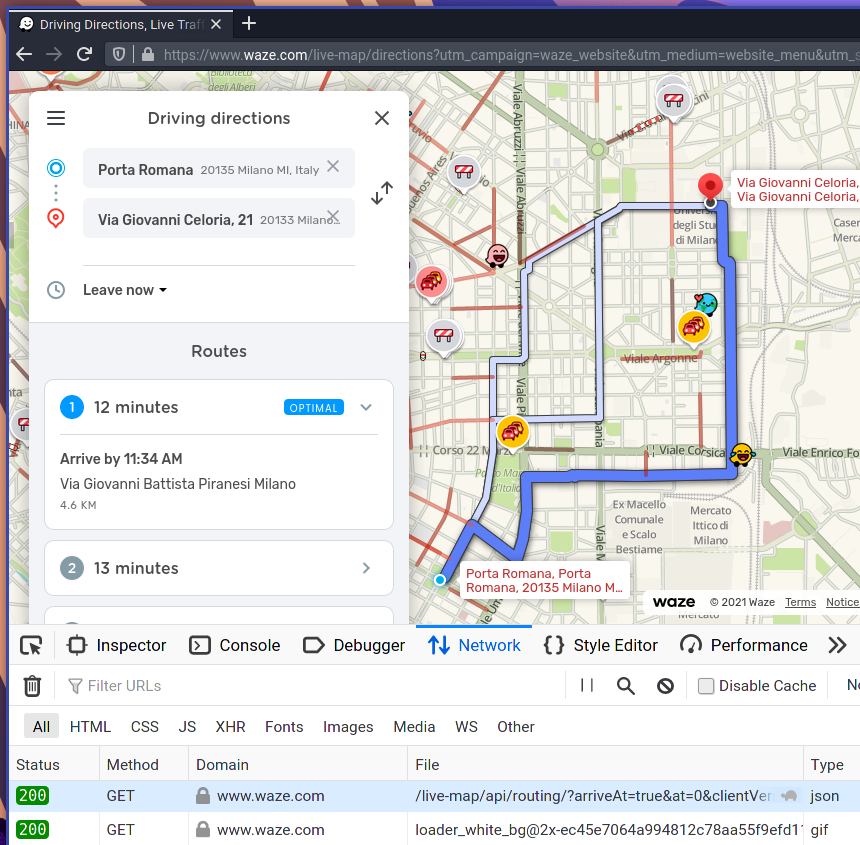
\includegraphics[scale=0.45]{waze_scraping}
	\caption{Console da sviluppatore su Firefox}
	\label{image:1}
\end{figure}
In particolare, la richiesta verso l'url \url{https://www.waze.com/live-map/routing/?} contiene esattamente il punto di partenza e di arrivo richiesti parametrizzati nell'url della richiesta, e il risultato è restituito è in formato JSON. Per proteggere i loro server da sovraccarichi, Waze risponde a questo URL solamente se si possiede il permesso ricevuto preventivamente tramite un token, ovvero una stringa di caratteri che funge da chiave segreta. Per ottenere questa chiave e raggiungere l'obbiettivo finale di avere delle API per interrogare il servizio, è stato scritto un programma in Golang per emulare l'interazione col sito web e ricevere il token necessario per effettuare le richieste successive. Questo processo ha richiesto tempo sia per la codifica dei parametri e che per la decodifica del risultato stesso e dei risultati intermedi per la richiesta del token. In altre parole, è stato fatto il reverse engineering della web app.

\subsection{Stima del percorso per il car sharing}

Avendo trovato un modo per risolvere i tempi di percorrenza in auto, per il servizio di car sharing Enjoy si è scelto di calcolare una stima che tiene conto del raggiungimento a piedi dell'auto libera più vicino al luogo di partenza del viaggio e del tragitto in auto tra la posizione di quest'ultima e il luogo di destinazione. Nello specifico, ogni volta che viene richiesto un percorso, viene scaricata la lista aggiornata delle auto libere presenti sul territorio e viene scelta l'auto più vicina calcolando la distanza dal punto di partenza richiesto a ogni auto presente nella lista. Una voltra trovata la posizone dell'auto libera, vengono sommate la stima di percorrenza del raggiungimento di tale auto a piedi e la stima di percorrenza in auto dal luogo in cui si trova l'auto fino alla destinazione. Sebbene non sia l'approccio migliore, dato che non tiene conto della direzione e del verso di marcia per compiere il viaggio, e quindi rendendo possibile la scelta di auto più vicina al punto di partenza ma che si allontana dal luogo di destinazione, è risultato il più semplice da programmare e successivamente da testare.

\section{Scelta tra percorsi random e prefissati}

Si è scelto di usare diverse tratte su cui basare il confronto allo scopo di ricoprire a livello topografico una buona parte del Comune di Milano e di diversificare i confronti in base alle caratteristiche delle tratte, quali lunghezza, coordinate geografiche di partenza e destinazione, per simulare al meglio la posizione di un possibile utente nella mappa.

Per rendere automatiche le richieste da inoltrare ai servizi di navigazione è stata creata una sorgente dal quale pescare le tratte. Sono stati presi in considerazione tre principali approcci per creare tale sorgente: hard-coded random; hard-coded di tratte realmente percorse; generazione a random just-in-time. I primi due approcci sono risultati fin da subito problematici.

In primo luogo, la scelta della destinazione avrebbe introdotto bias cognitivi riguardo il possibile utente del percorso, portando ad analizzare la mobilità solamente dal punto di vista di una determinata categoria, per esempio: selezionando tratte con delle università come punto di arrivo porterebbe ad analizzare la mobilità solamente dal punto di vista degli studenti e dipendenti presso quelle determinate strutture. Altri problemi simili sarebbero sorti nello scegliere la partenza, la lunghezza, la distanza dal centro città e numerosità delle tratte.

Seconda problematica molto più rilevante è che, involontariamente, si sarebbero introdotti dei percorsi che avrebbero favorito un mezzo piuttosto che un altro. Nella città di Milano infatti si contanto numerosi tratti stradali di questo genere: strade con corsia preferenziale per mezzi pubblici e taxi; strade a singola corsia e con numerosi semafori (quindi più soggetta a incolonnamenti); tangenziali; tratte coperte da passanti ferroviari (più veloci delle metropolitane e con meno fermate). Tale scelta avrebbe portato ad analizzare dati non rappresentativi della città, con conseguenti risultati in un certo senso "falsati".

Usando l'approccio della generazione a random non solo si sarebbero evitati tali problemi, ma i problemi stessi si sarebbero trasformati in analisi da poter eseguire a posteriori, per esempio selezionando da tutte le tratte generate a random quelle che hanno portato nei pressi di un'università, o tratte che in linea d'aria hanno coperto particolari strade favorevoli a determinati mezzi di trasporto. Visti i vantaggi e la flessibilità dell'approccio, si è optato per quest'ultimo.

\section{Generatore random dei percorsi}

Prima ancora di scrivere una funzione per generare tratte a random è stata scelta l'area geografica all'interno della quale generarle. Siccome il servizio di car sharing Enjoy non permette di usare la propria flotta al di fuori del Comune di Milano, tale area è stata selezionata come terreno per i confronti, rappresentata sotto forma di rettangolo per questioni di semplicità nella programmazione. Nello specifico, sono state scelte le coordinate (45.450562\textdegree, 9.158959\textdegree) e (45.482032\textdegree, 9.206763\textdegree) rispettivamente come vertice in basso a sinistra e in alto a destra del rettangolo rappresentativo dell'area selezionata. In questo modo la generazione di punti a random è stata ridotta alla generazione di coordinate maggiori o uguali della prima e minori o uguali della seconda.

Una volta scritta la funzione per la generazione a random delle tratte, è stato introdotto un constraint per simulare dei percorsi scomodi da fare a piedi, ovvero per generare tratte che supererebbero i 20 minuti di camminata per essere coperte, e al tempo stesso che giustificherebbero l'utilizzo della macchina. Si è scelto di usare 2 km in linea d'aria dal punto di partenza a quello di destinazione come misura minima della lunghezza di una tratta.

Un secondo constraint è stato introdotto per avere una maggiore eterogeneità delle tratte generate a livello geografico. Molte delle linee principali dei mezzi pubblici infatti attraversano il centro storico di Milano, inoltre l'area del centro storico rappresenta più della metà dell'area selezionata dal constraint precedente. Siccome è stato scelto di ricoprire a livello topografico tutta l'area di Milano, si è programmato il generatore in modo da creare in maniera equidistribuita le seguenti tipologie di tratte: da dentro il centro storico a fuori; da dentro a dentro; da fuori a fuori; da fuori a dentro. Il rettangolo rappresentativo del centro storico è stato disegnato secondo i seguenti vertici: (45.450562\textdegree, 9.158959\textdegree), (45.482032\textdegree, 9.206763\textdegree).

\section{Timing delle richieste}

Le richieste sono state programmate per essere effettuate dalle 7:00 alle 23:59 di ogni giorno. La scelta di tale intervallo è stata vincolata dall'orario di servizio dei mezzi pubblici ATM, difatti in tale orario viene garantito il pieno regime del servizio, mentre vengono offerti collegamenti e passaggi saltuari al di fuori di esso.
Per rispettare i limiti giornalieri delle varie API si è scelto di effettuare 1 richiesta al minuto, dove ogni richiesta rappresenta un tragitto generato a random mandato simultaneamente a ogni servizio di navigazione per ottenere una stima da ognuno di essi, per un totale di circa 1,000 richieste al giorno. Oltre ai valori delle stime di percorrenza per ogni mezzo, insieme alla richiesta sono stati salvati altri dati come il numero di macchine libere enjoy al momento della richiesta, la distanza aerea della tratta e quella calcolata a piedi. 

\section{Pseudocodice del programma}

\begin{lstlisting}[language=Go]
var a, b, c coordinate

for {
	a, b = creaTragittoRandom()
	c = enjoy.trovaAutoPiuVicinaOra(a)
	
	risultato := []stime{
		here.stimaTragitto(a, b),
		waze.stimaTragitto(a, b),
		osm.stimaTragitto(a, b, "foot"),
		osm.stimaTragitto(a, b, "bike"),
		osm.stimaTragitto(a, c, "foot") +
			waze.stimaTragitto(c, b)
	}
	
	save(risultato)
}
\end{lstlisting}

\chapter{Risultati}
\section{Raccolta dati}

I dati riguardanti la simulazione sono stati raccolti a partire dall'1 marzo 2020 fino al 27 giugno 2020 per un arco di tempo di circa 4 mesi, al ritmo di 1 richiesta al minuto dalle 7:00 alle 23:59 di ogni giorno.

\subsection{Le problematiche}

Sebbene questo studio fosse stato pensato per un confronto in condizioni di traffico e congestione stradale abituali che caratterizzano Milano, a influenzare questo studio è stato da subito l'emergenza epidemiologica da COVID-19. Il 22 gennaio 2020 il Governo Italiano ha dichiarato lo stato di emergenza, mettendo in atto le prime misure di contenimento in alcuni Comuni dove si sono verificati i primi casi del contagio. A partire dal 23 febbraio sono stati emanati DPCM (decreto del Presidente del Consiglio dei ministri) sempre più stringenti riguardo la circolazione e lo svolgimento delle attività commerciali, fino a ordinare un lockdown nazionale l'11 marzo 2020 \cite{misuredelgovernopercovid}. Nonostante lo studio sia stato fortemente influenzato da questo fattore, per via della circolazione ridotta se non totalmente assente durante il lockdown e per la riduzione del numero dei mezzi pubblici ATM, si è deciso comunque di procedere, tenendo conto dell'avvenuto sul giudizio finale dei risultati. A ostacolare lo studio, inoltre, nei primi giorni di utilizzo del programma per eseguire le richieste, è stato il servizio precedentemente utilizzato per i mezzi pubblici, ovvero Moovit, che ha risposto alle richieste con valori nulli o totalmente fuori scala. Per questo motivo è stato sostituito il servizio con quello offerto da Here e sono stati scartati i risultati precedentemente raccolti.

\subsection{Filtro dati errati}

I dati raccolti dalla prima esecuzione del programma, avvenuta l'1 marzo 2020, fino all'entrata in vigore dello stato di lockdown nazionale, il 12 marzo 2020, sono risultati per la maggior parte errati, ovvero con stime di percorrenza nulle, causati dai problemi con lo scraper di Moovit. Successivamente a questo evento si è cercato e trovato un servizio alternativo che sostituisse la stima del percorso coi mezzi pubblici, ovvero Here, che sfortunatamente non offre stime in tempo reale ma solo statiche. I dati raccolti nel periodo di lockdown dal 13 marzo 2020 al 3 maggio 2020 compresi sono stati scartati per via della circolazione dei mezzi pubblici e privati quasi totalmente assente, e quindi poco utili nell'obbiettivo finale dello studio di confrontare i mezzi di trasporto in situazioni di traffico caratteristico della città. Per questo motivo si è scelto di usare solamente i dati a partire dall'allentamento delle misure di restrizioni da emergenza sanitaria, ovvero quelli a partire dal 4 maggio 2020. Anche i dati presi in considerazione da quest'ultima data contengono delle stime nulle. Questo fenomeno è stato probabilmente dovuto alla generazione a random delle coordinate di partenza e arrivo, che ha permesso richieste in qualsiasi punto della mappa, compresi punti non situati direttamente sulla strada come in giardini pubblici, condomini e altre zone private, o semplicemente dovuto a disservizi. Per un confronto alla pari sono state considerate solo le righe prive di zeri nel file formato CSV. Come indicato dalla Tabella \ref{table:1} su circa 68000 richieste, 50000 sono prive di errori, circa il 73\% del totale, e quindi adatte per un confronto 1 a 1 tra mezzi di trasporto.

\begin{table}
	\centering
	\begin{tabular}{ | l | r | r | }
		\hline
		& \textbf{1 Marzo - 12 Marzo} & \textbf{4 Maggio - 27 Giugno} \\
		\hline
		\textbf{Coerenti}& 1988 & 49560 \\  
		\textbf{Errati} & 7962 & 18290 \\
		\hline
		\textbf{Totale} & 9680 & 67850 \\
		\textbf{\% Errati} & 79.5 & 27.0 \\
		\hline
	\end{tabular}
	\caption{Dati errati che contengono uno o più valori nulli nelle stime.}
	\label{table:1}
\end{table}

\subsection{Salvataggio}

Nella Tabella \ref{table:7} è riportato l'header del file CSV in cui sono stati salvati i dati. Nei campi di partenza e arrivo sono state salvate le coordinate espresse in gradi del tragitto generato, nei restanti campi le stime di percorrenza di tale tragitto espresse in minuti, insieme alla data e all'orario in cui è stata effettuata la richiesta di tale tratta. Oltre ai dati principali sono state salvate informazioni secondarie come il numero di auto libere Enjoy al momento della richiesta, la lunghezza in via aerea della tratta e quella totale del percorso di ogni mezzo, tutte espresse in chilometri.

\begin{table}[H]
	\centering
	\begin{tabular}{ | c | c | c | c | c | c | c | c | c | }
		\hline
		Data & Orario & Partenza & Arrivo & Auto & ATM & Enjoy & Bici & Piedi \\
		\hline
	\end{tabular}
	\caption{Header del file CSV con i dati salvati.}
	\label{table:7}
\end{table}

\subsection{Distribuzione lunghezza tratte generate}

Nella Figura \ref{image:2} e nella Tabella \ref{table:2} sono riportate le statistiche riguardo la lunghezza in via aerea delle tratte generate. Si può notare come più della metà siano lunghe meno di 5 km in linea aerea, risultato voluto e ottenuto dai vincoli imposti nella generazione riguardanti l'area del Comune di Milano e per l'ingresso e l'uscita dal centro storico al semicentro. La Figura \ref{image:19} mostra come la lunghezza delle tratte è stata equidistribuita nelle diverse fasce di orario.

\begin{figure}[H]
	\centering
	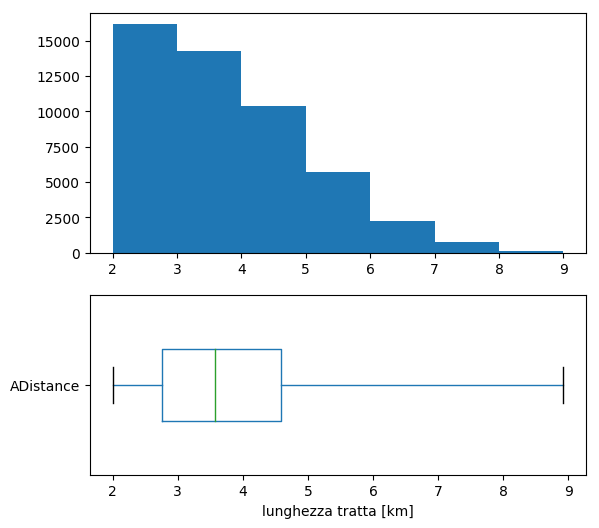
\includegraphics[scale=0.8]{distribuzione_tratte}
	\caption{Frequenza assoluta e distribuzione lunghezza tratte [km].}
	\label{image:2}
\end{figure}

\begin{figure}[H]
	\centering
	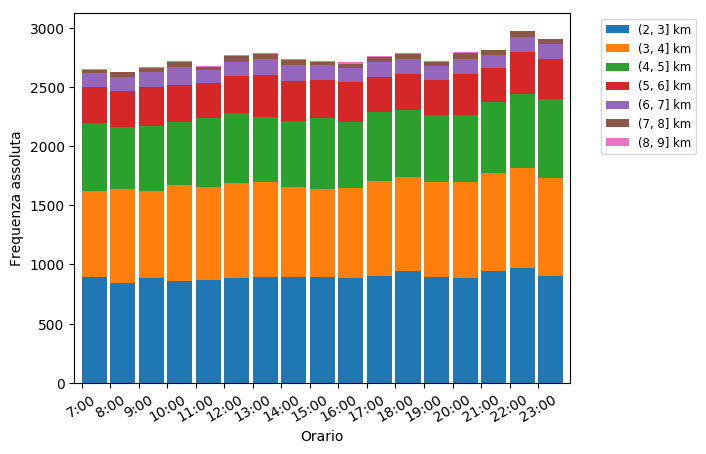
\includegraphics[scale=0.8]{distribuzione_tratte_oraria}
	\caption{Frequenza assoluta lunghezza tratte in base all'orario [km].}
	\label{image:19}
\end{figure}

\begin{table}[H]
	\centering
	\begin{tabular}{ | l r | }
		\hline
		\textbf{Abs. freq.} & 49560 \\
		\textbf{Media} & 3.80 km \\
		\textbf{Mediana} & 3.57 km \\
		\textbf{Std} & 1.27 km \\
		\textbf{Min} & 2.00 km \\
		\textbf{Max} & 9.52 km \\
		\hline
	\end{tabular}
	\caption{Statistiche lunghezza tratta [km].}
	\label{table:2}
\end{table}

\section{Performance dei singoli mezzi}

Dalla Figura  \ref{image:26} si può subito notare come i tragitti a piedi e in bicicletta abbiano dei baffi molto corti se non totalmente assenti rispetto agli altri mezzi, con conseguente varianza molto bassa, il che è un risultato aspettato dato che non c'è nessun fattore oltre la distanza a influenzare drasticamente il tempo di percorrenza per questi metodi di spostamento, motivo per cui i provider si limitano a calcolarne una stima statica.

\begin{table}
	\centering
	\begin{tabular}{ | l r r r r r | }
		\hline
		& \textbf{Auto} & \textbf{Enjoy} & \textbf{Bici} & \textbf{ATM} & \textbf{Piedi} \\
		\textbf{Media}      & 23.7 & 16.4 & 11.9 & 10.3 & 4.5 \\
		\textbf{Mediana} & 23.6 & 16.2 & 11.9 &   9.8 & 4.5 \\
		\textbf{Std}             &  3.9 &   4.2 &   1.3 &    3.0 & 0.0 \\
		\textbf{Min}            &  8.9 &   3.5 &   6.5 &    3.7 & 4.3 \\
		\textbf{Max}         & 59.0 & 46.4 & 16.9 &  41.0 & 4.6 \\
		\hline
	\end{tabular}
	\caption{Statistiche velocità media [km/h].}
	\label{table:3}
\end{table}

 Risultato opposto invece è stato ottenuto per i tragitti in auto, car sharing e mezzi pubblici, che mostrano una varianza molto più alta, come riportato nella Tabella \ref{table:3}, dovuta alla presenza di diverse variabili nel calcolo del tragitto. Nonostante le stime di percorrenza dei mezzi pubblici siano state calcolate dal provider usando solamente le tabelle degli orari dei mezzi, la varianza è risultata comunque alta per via delle numerosi variabili che influiscono sul tempo di percorrenza, come la distanza tra il punto di partenza e la fermata del mezzo, la scelta stessa del tipo di mezzo, come bus, tram o metro, e la corrispettiva velocità nominale. Questi primi risultati sono in linea con quelli dell'ISFORT riportati nella Tabella \ref{table:9}, che vede l'automobile in testa alla classifica intorno a 22 km/h di media, con la bici al secondo posto ma con 15 km/h e i mezzi pubblici al terzo con 14 km/h, stime poco più alte di quelle sopra riportate.

\begin{figure}
\centering
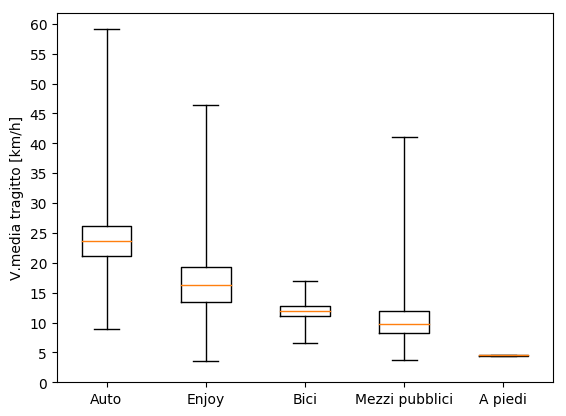
\includegraphics[scale=0.7]{vmedia_all}
\caption{Distribuzione velocità media dei singoli mezzi.}
\label{image:26}
\end{figure}

\pagebreak

\subsection{Automobile}

\subsubsection{Velocità media}

Una delle prime analisi effettuate per ogni mezzo è stata quella di calcolare la velocità media per ogni tragitto effettuato riguardante l'intero periodo di raccolta dati, con l'obbiettivo di osservare eventuali variazioni di ora in ora. Come riportato nella Figura \ref{image:3}, si evidenziano due situazioni, caratterizzate da una differenza nella velocità media: più bassa nelle fasce di orario delle 8:00-11:00 e delle 17:00-19:00, in cui è stata registra la velocità media minima di 23 km/h, e più alta nelle ore restanti. La massima velocità media invece è stata rileva nei tragitti dopo le 22:00, di circa 26 km/h. Tali risultati sono in linea, tra i tanti studi a riguardo del traffico in auto a Milano, con quelli dello studio di TomTom\footnote{\url{https://www.tomtom.com/en_gb/traffic-index/ranking/}. Accessed: 20/01/2021} effettuato sulla città di Milano nel 2019, che evidenzia le 9:00 e le 18:00 come orari di picco del traffico stradale dal lunedì al venerdì, con un livello di congestione rispettivamente del 70\% e del 60\%.

\begin{figure}[H]
	\centering
	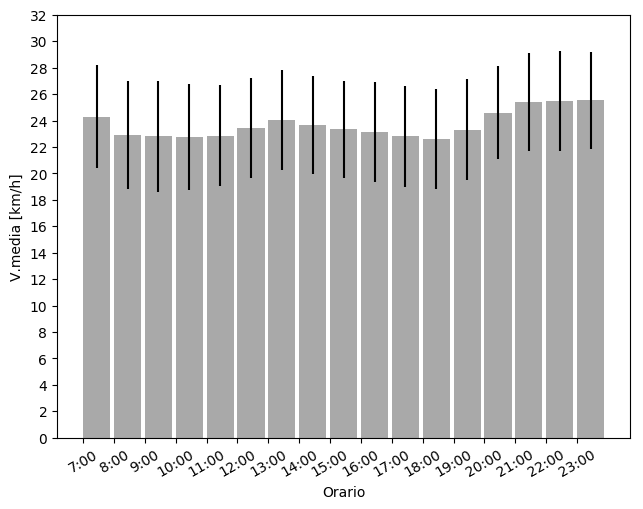
\includegraphics[scale=0.8]{vmedia_oraria_auto}
	\caption{Velocità media in auto [km/h] di ora in ora. I baffi neri rappresentano la deviazione standard campionaria $\sigma$ rispettiva di ogni barra.}
	\label{image:3}
\end{figure}

Risultano in linea con lo studio anche le ore precedenti e successive agli orari individuati come picchi. Si nota inoltre come le deviazioni standard campionarie di ogni ora, rappresentate da baffi neri incastonati nelle barre, rimangano invariate. Si è scelto di rappresentare la deviazione standard invece che l'errore standard per via dell'elevata numerosità del campione che renderebbe i baffi non visibili e quindi non distinguibili. Difatti, basandosi sui dati della Tabella \ref{table:3} che riporta una deviazione standard di 3.9 e nella Figura \ref{image:19} che mostra una media di circa 2600 tratte per ogni fascia di orario, l'errore standard per ogni barra risulterebbe di: $\frac{\sigma_x}{\sqrt{n}} = \frac{3.9}{\sqrt{2600}} = 0.07$.



\subsubsection{Velocità media lunedì-venerdì e sabato-domenica}

La Figura \ref{image:4} mostra il risultato di una ripartizione dei dati effettuata sulla base del giorno della settimana, in particolare sono stati divisi i tragitti effettuati dal lunedì al venerdì da quelli del sabato e domenica. Per rendere leggibile la differenza è stata spostata l'origine del grafico al valore 16 sull'asse delle ordinate. 

\begin{figure}[H]
	\centering
	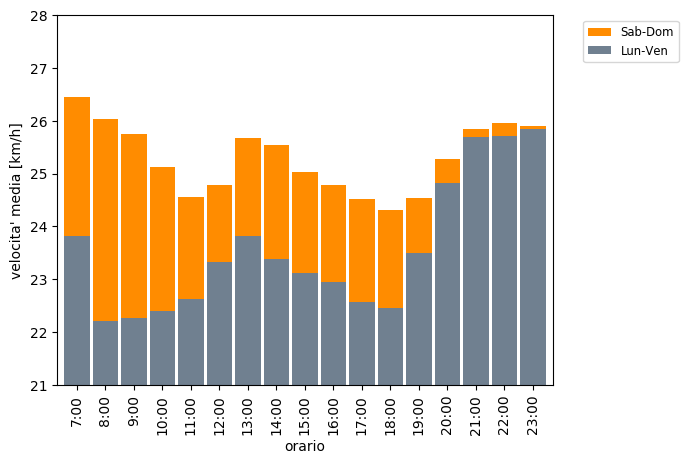
\includegraphics[scale=0.8]{vmedia_oraria_auto_weekend}
	\caption{Velocità media in auto [km/h] di ora in ora. I valori sull'asse delle ordinate variano tra 16 e 28.}
	\label{image:4}
\end{figure}

La differenza è nel complesso bassa, di circa 2 km/h di media, che tende a diminuire nel primo pomeriggio e negli orari notturni e ad aumentare nella fascia oraria delle ore 8;00 e delle 16:00, con una differenza di quasi 4 km/h, equivalente a un incremento della velocità media nel fine settimana del 14.6\% in più rispetto al lunedì-venerdì. La variazione della velocità media di ora in ora nel sabato-domenica risulta meno evidente di quella del lunedì-venerdì, con i picchi di rallentamento che si spostato nelle fasce orarie 10:00-12:00 e 16:00-19:00. Anche questi dati risultano in linea con quelli dello studio di TomTom, che vede un minor livello di congestione nel weekend con dei picchi nelle ore 10:00 e 18:00. La deviazione standard delle fasce di orario del lunedì-venerdì e sabato-domenica, che sono state omesse per motivi di leggibilità del grafico, rimangono sempre costanti intorno al valore 3.7 km/h, con un errore standard di $\frac{3.7}{\sqrt{1622}} = 0.09$ per i giorni dal lunedì al venerdì e $\frac{3.7}{\sqrt{622}} = 0.14$ per i fine settimana, dove 1622 e 622 rappresentano rispettivamente la numerosità del campione di una sola fascia di orario lunedì-venerdì e di sabato-domenica.

\subsubsection{Velocità media settimana dopo settimana da fine lockdown}

La Figura \ref{image:5} mostra il risultato di una ripartizione dei dati effettuata in base alla settimana, in particolare sono stati partizionati a gruppi di 2 settimane consecutive i tragitti effettuati a partire dal 4 maggio 2020, primo giorno dell'allentamento delle restrizioni imposte dal governo italiano per l'emergenza COVID-19 \cite{misuredelgovernopercovid}. Nel grafico risulta evidente una degradazione della velocità media generale e lineare rispetto al passare delle settimane. Si nota inoltre che le curve corrispondenti alle settimane successive al 17 maggio, ovvero dopo le prime 2, presentino dei flessi sempre più accentuati in prossimità degli orari di picco del traffico evidenziati dalla Figura \ref{image:3}. Anche in questo caso, non sono state riportate differenze nella deviazione standard. Nella Figura \ref{image:27} sono stati usati i box plot per descrivere la distribuzione delle velocità medie a gruppi di 2 settimane dalla fine del lockdown. Si può notare come il quartile zero, primo, secondo e terzo siano rimasti uguali, con un lieve andamento a ribasso col passare delle settimane. La differenza risulta più accentuata nel quarto quartile, che vede la diminuzione dei valori di massima velocità media per tragitto, probabilmente dovuta a un aumento del traffico, come emerso dal grafico della Figura \ref{image:5} con valori decrescenti della velocità media per ogni fascia di orario al passare delle settimane dalla fine del lockdown.

\begin{figure}
	\centering
	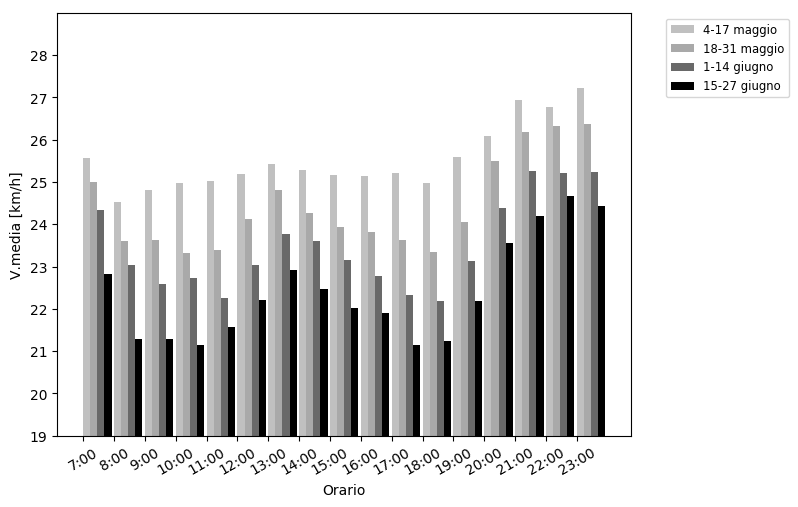
\includegraphics[scale=0.8]{vmedia_oraria_auto_weeks}
	\caption{Velocità media in auto [km/h] di ora in ora. I valori sull'asse delle ordinate variano tra 16 e 30.}
	\label{image:5}
\end{figure}

\begin{figure}
	\centering
	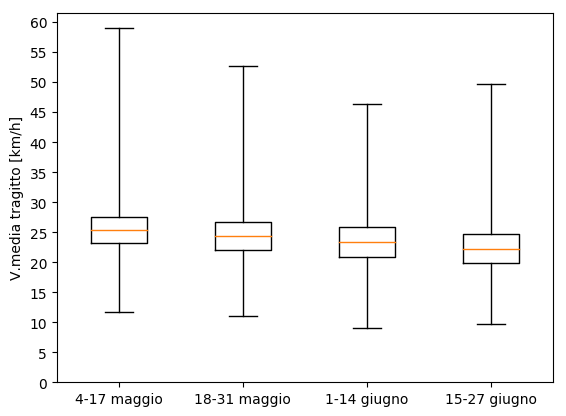
\includegraphics[scale=0.8]{vmedia_auto_weeks}
	\caption{Distribuzione della velocità media in auto [km/h] calcolata a gruppi di 2 settimane dalla fine del lockdown.}
	\label{image:27}
\end{figure}

\begin{figure}[H]
	\centering
	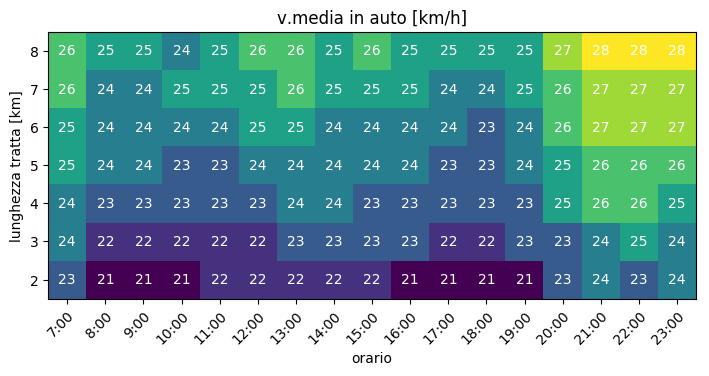
\includegraphics[scale=0.75]{heatmap_auto}
	\caption{Velocità media in auto [km/h] di ora in ora in base alla lunghezza della tratta.}
	\label{image:6}
\end{figure}

\subsubsection{Velocità media in base alla lunghezza del tragitto}

Nella Figura \ref{image:6} sono riportati, tramite una heatmap, i dati della velocità media divisi per fasce d'orario e per lunghezza della tratta. Si evidenziano due gobbe in corrispondenza degli orari di picco del traffico intorno alle ore 9:00 e 18:00, e le tratte brevi, lunghe dai 2 ai 3 chilometri, risultano le più colpite. Si evidenzia inoltre un'area di forma rettangolare di colori chiari a partire dalle ore 20:00, dove la velocità media si stabilizza intorno ai 27 km/h per le tratte superiori ai 3 km.



\pagebreak

\subsection{Enjoy}

\subsubsection{Velocità media}

I tragitti col servizio di car sharing Enjoy hanno subito una lieve variazione di velocità media nell'arco 8:00-11:00 e in quello delle 17:00-19:00 in cui si è registrata la velocità media minima di 16 km/h e di 17 km/h di massima. La variazione è all'atto pratico poco significativa. La deviazione standard rimane costante per tutte le fasce di orario. Rispetto al grafico della Figura \ref{image:3} della velocità media in auto, la curva risulta molto simile, traslata verticalmente di 6 km/h. Anche in questo caso è stata usata la deviazione standard invece dell'errore standard per motivi di leggibilità, data l'elevata numerosità del campione.

\begin{figure}[H]
	\centering
	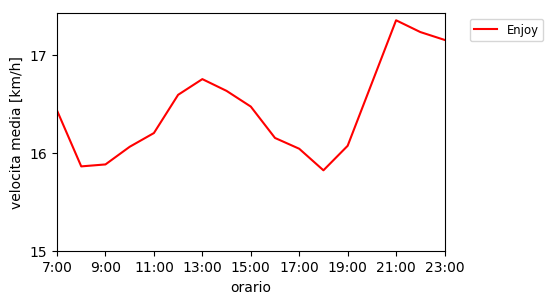
\includegraphics[scale=0.8]{vmedia_oraria_enjoy}
	\caption{Velocità media usando il car sharing Enjoy [km/h] di ora in ora.  I baffi neri rappresentano la deviazione standard campionaria $\sigma$ rispettiva di ogni barra.}
	\label{image:7}
\end{figure}

\subsubsection{Velocità media lunedì-venerdì e sabato-domenica}

Non sono state registrate particolari differenze effettuando la ripartizione dei dati in base ai giorni dal lunedì al venerdì e del fine settimana, come mostrato nella Figura \ref{image:20}. La velocità media rimane costante, con una lieve differenza nella fascia oraria delle 8:00. La deviazione standard, rimane costante e identica a quella della Figura \ref{image:7} per tutte le fasce di orario.

\begin{figure}[H]
	\centering
	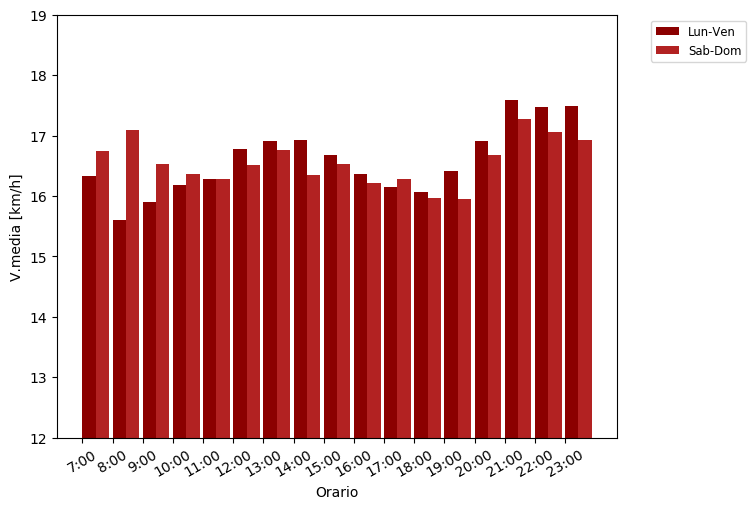
\includegraphics[scale=0.8]{vmedia_oraria_enjoy_weekend}
	\caption{Velocità media usando il car sharing Enjoy [km/h] di ora in ora. I valori sull'asse delle ordinate variano tra 12 e 21.}
	\label{image:20}
\end{figure}

\subsubsection{Velocità media settimana dopo settimana da fine lockdown}

Anche per il car sharing risulta evidente una degradazione della velocità media generale e lineare rispetto al passare delle settimane, come riportato nel grafico della Figura \ref{image:16}. Non risultano differenze nelle fasce orarie meno trafficate dalle 12:00 alle 15:00 e dalle 21:00 alle 23:00. Le prime due settimane dall'allentamento delle restrizioni risultano più veloci di circa 1 km/h di media dalle altre settimane. Nel grafico della Figura \ref{image:28}, come per l'automobile di proprietà, il quartile zero, primo, secondo e terzo risultano uguali, con un andamento decrescente del baffo del quarto quartile entro cui ricadono i valori massimi di velocità media per tragitto, sempre dovuto con molta probabilità al traffico.

\begin{figure}[H]
	\centering
	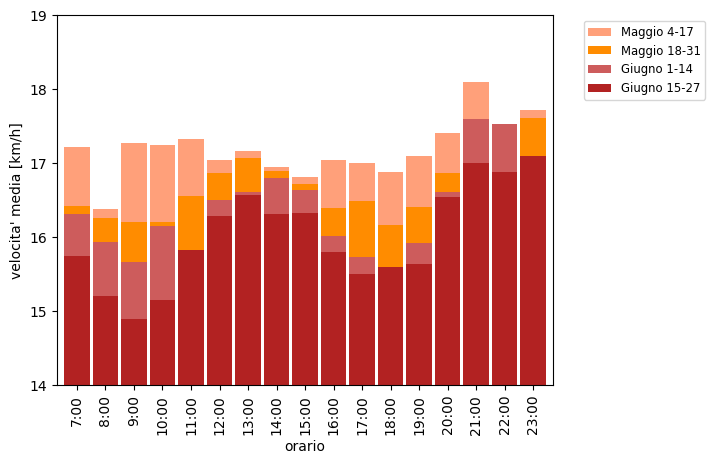
\includegraphics[scale=0.8]{vmedia_oraria_enjoy_weeks}
	\caption{Velocità media in car sharing Enjoy [km/h] di ora in ora. I valori sull'asse delle ordinate variano tra 12 e 21.}
	\label{image:16}
\end{figure}

\begin{figure}
	\centering
	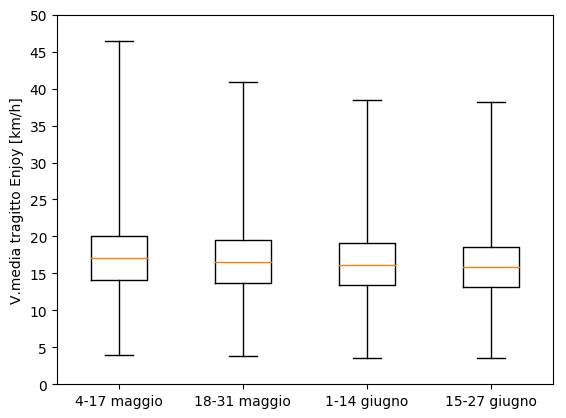
\includegraphics[scale=0.8]{vmedia_enjoy_weeks}
	\caption{Distribuzione della velocità media in car sharing Enjoy [km/h] calcolata a gruppi di 2 settimane dalla fine del lockdown.}
	\label{image:28}
\end{figure}

\subsubsection{Velocità media in base alla lunghezza del tragitto}

Nel grafico della Figura \ref{image:30} sono riportati, tramite una heatmap, i dati della velocità media divisi per fasce d'orario e per lunghezza della tratta. In questo caso, a differenza della heatmap dell'auto di proprietà, corrispondente alla Figura \ref{image:6}, le velocità medie risultano mediamente costanti in base alla lunghezza della tratta, indipendentemente dall'orario, con lievi diminuzioni nelle ore intorno alle 9:00 e 18:00. A differenza dell'auto, la velocità media sembra non aumentare in corrispondenza degli orari notturni, questo probabilmente è dovuto al grande impatto che ha il tratto a piedi per raggiungere un mezzo libero della flotta.

\begin{figure}
	\centering
	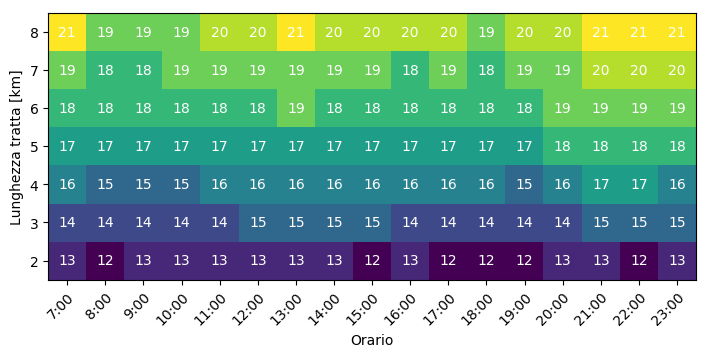
\includegraphics[scale=0.75]{heatmap_enjoy}
	\caption{Velocità media in car sharing Enjoy [km/h] di ora in ora in base alla lunghezza della tratta.}
	\label{image:30}
\end{figure}

\subsubsection{Auto libere e tempo medio per raggiungerle}

Sottraendo il tempo impiegato in auto da quello impiegato col car sharing Enjoy è stata ottenuta una stima indicativa del tempo medio per raggiungere un'auto libera a piedi. Dai calcoli è risultato che il tempo medio oscilla intorno ai 6 minuti, come riportato dalla Tabella \ref{table:4}. Il box plot della Figura \ref{image:8} evidenzia il range interquartile nell'intervallo dai 3 ai 9 minuti, con una mediana di 6. Il tempo medio per raggiungere un'auto Enjoy, di 6.6 minuti, sembra coincidere con la differenza di velocità media rispetto ai dati dell'auto privata, citata a riguardo del grafico della Figura \ref{image:7}.

Anche per questa analisi i dati sono stati partizionati per i giorni da lunedì a venerdì e per sabato e domenica. Il grafico della Figura \ref{image:21} mostra una lieve differenza nel tempo medio per raggiungere un'auto libera Enjoy di circa 1 minuto a sfavore dei giorni del fine settimana. Dunque, in settimana, le auto sono risultate più facilmente raggiungibili.

Per contestualizzare il tempo medio per raggiungere un'auto Enjoy è stato usato il dato sul numero delle auto libere salvato per ogni richiesta ai servizi. Il massimo numero di auto libere in circolazione è stato di 870. Nella Figura \ref{image:9} viene mostrata in media la variazione di questo conteggio lungo l'arco della giornata, ripartito per lunedì-venerdì e sabato-domenica. Si può notare come il picco di utilizzo del servizio, denotato da un calo delle auto libere a disposizione, inizia verso le 15:00 e finisce verso le 21:00 indipendentemente dal giorno. L'unica differenza tra i due gruppi si può notare nelle ore del mattino, che vede meno auto libere durante la settimana. Il grafico della Figura \ref{image:10} mostra chiaramente come il numero delle auto libere a disposizione sia aumentato con la fine del lockdown. Si può notare infatti come siano state immesse circa 150 nuove auto nell'arco di un mese e altre 50 nel mese successivo. Questo dato è stato probabilmente dovuto al ritiro di una parte del parco auto da parte delle aziende per motivi di manutenzione, vista l'occasione della scarsa domanda di servizio.

\begin{table}[H]
	\centering
	\begin{tabular}{ | l r | }
		\hline
		& \textbf{T.medio ragg.auto} \\
		\textbf{Media}   &  6.6 \\
		\textbf{Mediana} &  6.0 \\
		\textbf{Std}     &  4.6 \\
		\textbf{Min}     &  0.0 \\ 
		\textbf{Max}     & 43.0 \\
		\hline
	\end{tabular}
	\caption{Statistiche tempo medio per raggiungere auto libera [min].}
	\label{table:4}
\end{table}

\begin{figure}[H]
	\centering
	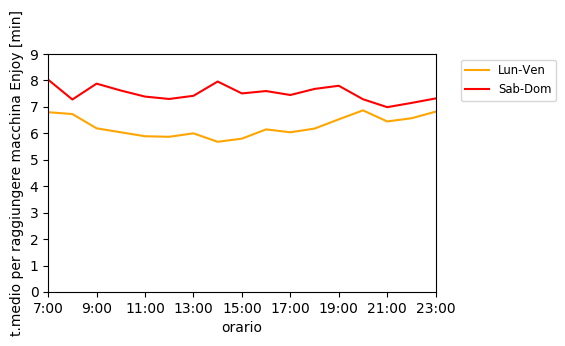
\includegraphics[scale=0.7]{tmedio_raggiungimento_auto_enjoy}
	\caption{Distribuzione del tempo impiegato a raggiungere auto libera [min].}
	\label{image:8}
\end{figure}

\begin{figure}
	\centering
	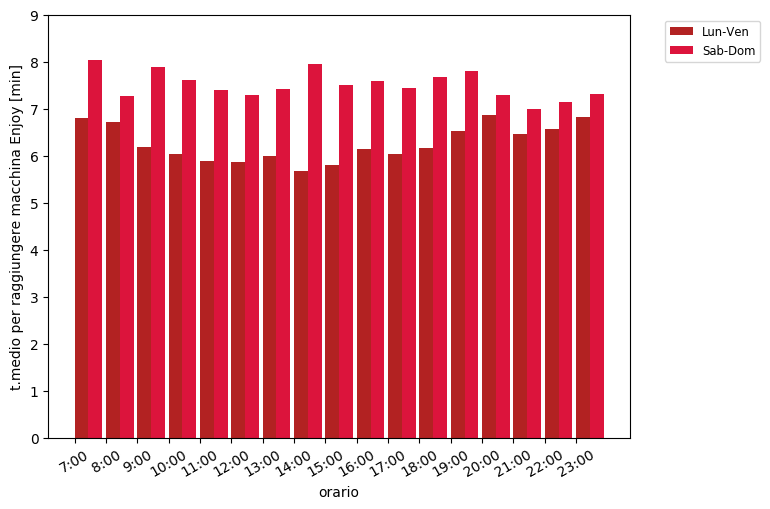
\includegraphics[scale=0.8]{tmedio_raggiungimento_auto_enjoy_weekend}
	\caption{Tempo medio per raggiungere auto libera [min].}
	\label{image:21}
\end{figure}

\begin{figure}
	\centering
	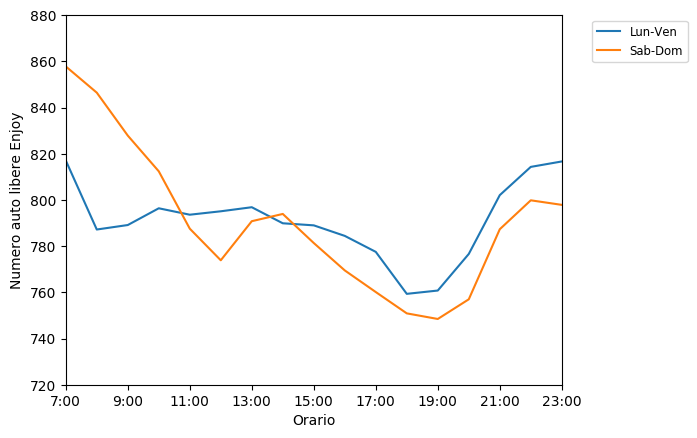
\includegraphics[scale=0.8]{variazione_auto_libere_enjoy_weekend}
	\caption{Numero di auto libere Enjoy lungo l'arco della giornata.}
	\label{image:9}
\end{figure}

\begin{figure}
\centering
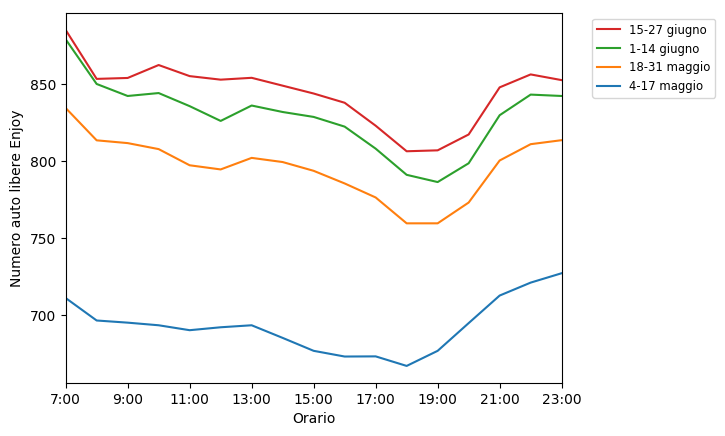
\includegraphics[scale=0.8]{variazione_auto_libere_enjoy_weeks}
\caption{Numero di auto libere Enjoy lungo settimana dopo settimana.}
\label{image:10}
\end{figure}

\pagebreak

\subsection{Mezzi pubblici ATM, bici e a piedi}

Analizzando le stime di percorrenza riguardo i mezzi pubblici, la bicicletta e i percorsi a piedi, non si è verificata alcuna variazione significativa lungo l'arco della giornata, tradotto graficamente come nelle Figure \ref{image:11}, \ref{image:17} e \ref{image:18} in una retta parallela all'asse x per ognuno dei mezzi considerati. Il risultato è aspettato, dato che tali servizi non hanno fornito risposte dinamiche in base alle condizioni attuali del traffico e dei dati storici, e, nel caso della bicicletta e a piedi, perché l'influenza è praticamente nulla per questi mezzi di trasporto.

Si è deciso di analizzare ulteriormente le performance dei mezzi pubblici per via della loro grande varianza, al pari di quella dell'auto e del car sharing. Nel grafico della Figura \ref{image:29} è riportata un'analisi tramite box plot per visualizzare la distribuzione dei valori di velocità media di settimana in settimana dalla fine del lockdown. Dal risultato emerge un netto cambiamento del quarto quartile a partire dal 1 giugno 2020, che vede un accorciamento del baffo corrispondente ai valori massimi di velocità media registrati. Nel tentativo di trovare una risposta a questo cambiamento, dato che può dipendere solamente dal cambio delle tabelle degli orari dei mezzi, visto che le API Here usate per questo mezzo si basano solo su di esse, si è tentato di accedere agli archivi pubblici delle notizie riguardanti cambiamenti di servizio dal sito dell'azienda fornitrice ATM, ma al momento della scrittura questa pagina risulta inaccessibile per via di un errore interno del server\footnote{\url{https://atm.it/it/AtmNews/AtmInforma/}. Accessed: 20/01/2021}.

\begin{figure}[H]
	\centering
	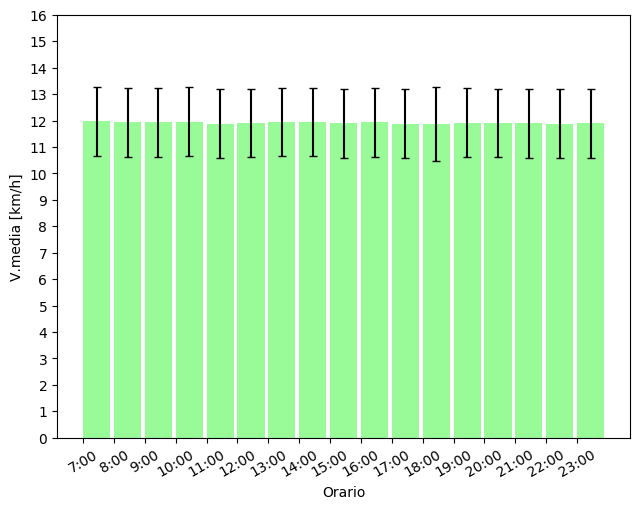
\includegraphics[scale=0.6]{vmedia_oraria_bici}
	\caption{Velocità media in bici [km/h] di ora in ora. I baffi neri rappresentano la deviazione standard campionaria $\sigma$ rispettiva di ogni barra.}
	\label{image:11}
\end{figure}

\begin{figure}[H]
	\centering
	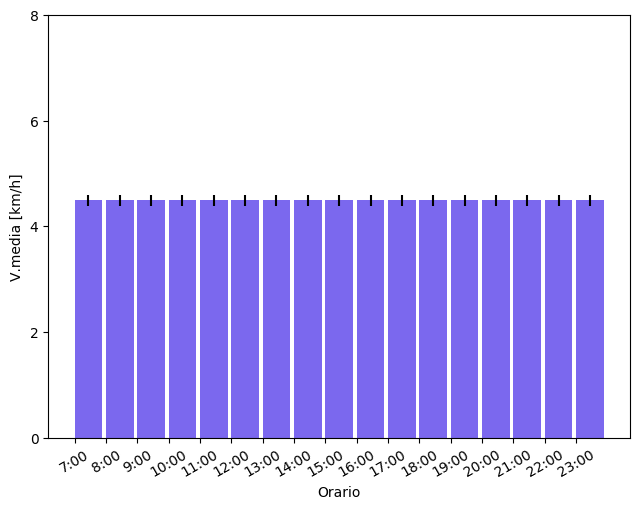
\includegraphics[scale=0.6]{vmedia_oraria_piedi}
	\caption{Velocità media a piedi [km/h] di ora in ora. I baffi neri rappresentano la deviazione standard campionaria $\sigma$ rispettiva di ogni barra.}
	\label{image:18}
\end{figure}

\begin{figure}
\centering
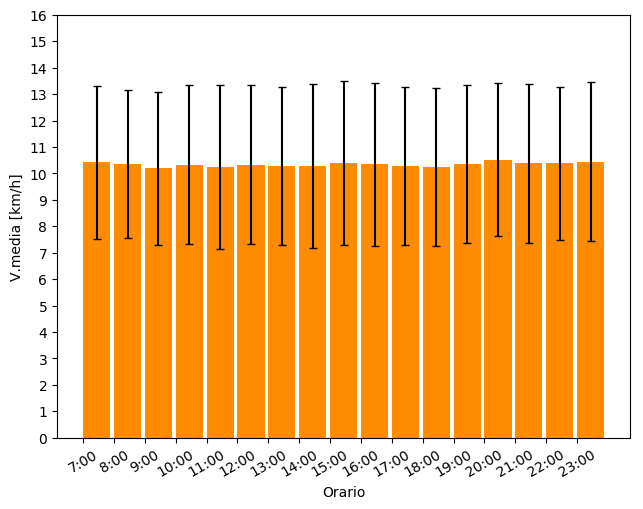
\includegraphics[scale=0.7]{vmedia_oraria_atm}
\caption{Velocità media coi mezzi pubblici [km/h] di ora in ora. I baffi neri rappresentano la deviazione standard campionaria $\sigma$ rispettiva di ogni barra.}
\label{image:17}
\end{figure}

\begin{figure}
\centering
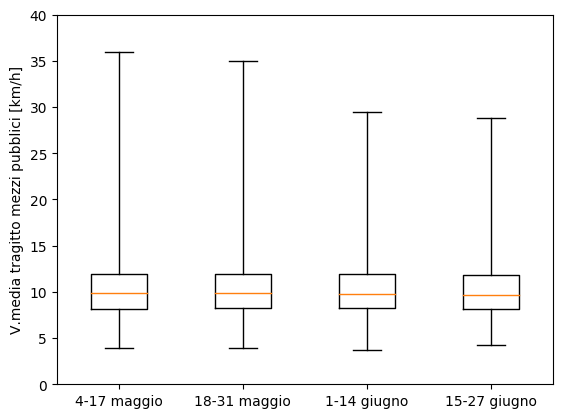
\includegraphics[scale=0.7]{vmedia_atm_weeks}
\caption{Distribuzione della velocità media coi mezzi pubblici [km/h] calcolata a gruppi di 2 settimane dalla fine del lockdown.}
\label{image:29}
\end{figure}


\section{Confronto tra mezzi}

In questo paragrafo sono stati raccolti i risultati più interessanti emersi dal confronto tra tutti i mezzi di trasporto a disposizione per spostarsi nel Comune di Milano. Il confronto più atteso che ha fatto da guida verso questo studio è stato quello di verificare se, per un uso interno al Comune di Milano a solo scopo di spostamento e senza vincoli particolari come trasporto merci o passeggeri, l'automobile privata, insieme ai suoi svantaggi, potesse essere surclassata da un mezzo più economico e pulito come i mezzi pubblici in una città dove il traffico influisce in buona parte sui tempi di percorrenza, come mostrato nella Figura \ref{image:22}.

\subsection{Vittoria dell'automobile}

Nonostante la grande influenza del traffico sui tempi di percorrenza, i tragitti in auto sono risultati sempre i più veloci di ogni sua controparte, a qualsiasi ora del giorno e su ogni distanza, con una vittoria sopra il 99\% delle volte.

\subsection{Parziale sconfitta del car sharing}

\subsubsection{Mezzi pubblici ATM vs. Enjoy}

I risultati del confronto tra i mezzi pubblici ATM e il servizio di car sharing Enjoy illustrati nella Tabella \ref{table:5} mostrano una percentuale di vittorie di circa il 9\%, dove per vittoria si intende che il tempo impiegato a percorrere una tratta coi mezzi pubblici è stato minore o uguale al tempo impiegato utilizzando il car sharing. Nel grafico della Figura \ref{image:13} viene visualizzata la distribuzione di queste vittorie di ora in ora. Si può notare come vicino alle ore di picco del traffico individuate nell'analisi delle performance dell'auto, ovvero le ore 8:00-10:00 e 17:00-20:00, si concentri la percentuale maggiore di sconfitte da parte del car sharing. Per esempio, su tutte le tratte richieste nelle ore 8:00, nell'11\% delle volte i mezzi pubblici hanno pareggiato o superato la performance del car sharing. Al contrario, al di fuori degli orari di picco del traffico, la percentuale di vittorie è vicina allo 0. Dalla Tabella \ref{table:5} si evince anche che dell'8.7\% di queste vittorie, circa metà di esse sono tratte brevi dai 2 ai 5 km.

\subsubsection{Bicicletta vs. Enjoy}

Risultato ancora più interessante è quello del confronto tra bicicletta di proprietà e car sharing. La tabella \ref{table:6} mostra una percentuale delle vittorie del 36\% sul totale, poco più di un terzo del totale delle tratte. La maggior parte di queste vittorie è concentrata nelle tratte brevi dai 2 ai 5 km. Anche in questo confronto è emerso che negli orari di picco si accentua la percentuale di vittorie che arriva a toccare quasi il 45\% del totale nelle ore 8:00 e 18:00 come riportato dal grafico della Figura \ref{image:14}. Al contrario dei mezzi pubblici, questa percentuale resta alta anche al di fuori degli orari di punta, restando sempre intorno al 30\%.

\begin{table}[H]
	\centering
	\begin{tabular}{ | r r r | }
		\hline
		& \textbf{Abs. freq.} & \textbf{\% win} \\
		\textbf{(2, 5] km} & 2072 & 4.2 \\
		\textbf{(5, 7] km} & 1512 & 3.1 \\
		\textbf{(7, 10] km} & 670 & 1.4 \\
		\hline
		\textbf{totale} & 4294 & 8.7 \\
		\hline
	\end{tabular}
	\caption{Vittoria dei mezzi pubblici su Enjoy per lunghezza tratta.}
	\label{table:5}
\end{table}

\begin{figure}[H]
	\centering
	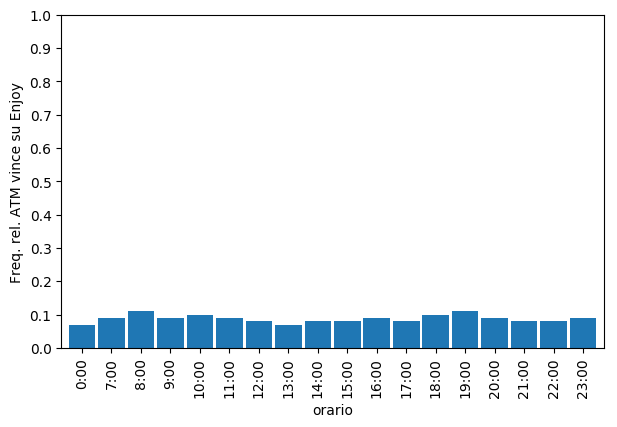
\includegraphics[scale=0.7]{confronto_atm_enjoy}
	\caption{Frequenza relativa vittorie ATM su Enjoy di ora in ora.}
	\label{image:13}
\end{figure}

\pagebreak

\begin{table}[H]
	\centering
	\begin{tabular}{ | r r r | }
		\hline
		& \textbf{Abs. freq.} & \textbf{\% win} \\
		\textbf{(2, 5] km} & 15215 & 30.7 \\
		\textbf{(5, 7] km} & 2423 & 4.9 \\
		\textbf{(7, 10] km} & 278 & 0.6 \\
		\hline
		\textbf{totale} & 17917 & 36.2 \\
		\hline
	\end{tabular}
	\caption{Vittoria della bicicletta su Enjoy per lunghezza tratta.}
	\label{table:6}
\end{table}

\begin{figure}[H]
	\centering
	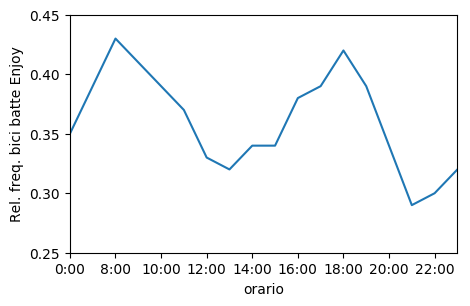
\includegraphics[scale=0.7]{confronto_bike_enjoy}
	\caption{Frequenza relativa vittorie bicicletta su Enjoy di ora in ora.}
	\label{image:14}
\end{figure}

\pagebreak

\section{Confronto pre e post lockdown}

Nonostante le prime versioni del programma di raccolta dati abbiano portato a diversi errori nelle stime, quelle relative al percorso in automobile e car sharing sono sempre state corrette. Si è deciso quindi di analizzare l'unica settimana a disposizione prima del lockdown, dal lunedì 2 a domenica 8 marzo 2020, con una delle settimane più trafficate dopo il lockdown, che dalle analisi riportate dalle Figure \ref{image:5} e \ref{image:16} sono risultate corrispondenti al periodo dal 15 al 27 giugno 2020.

\subsection{Automobile}

Nel grafico della Figura \ref{image:22} si può notare una lieve differenza di km/h di media tra una settimana pre e post lockdown dal lunedì al venerdì. Questa differenza risulta più evidente negli orari di picco del traffico vicino alle 8:00 e alle 18:00, con una differenza di 2 km/h di media. Risulta evidente inoltre la differenza di velocità media nel pre lockdown tra le ore 8:00, dove si tocca il minimo di 17.5 km/h, e le ore 23:00, dove si trova il massimo di 24.5 km/h, una differenza di velocità del 28\%.

\subsection{Enjoy}

I tempi di percorrenza in car sharing Enjoy sono risultati molto simili, come mostrato dal grafico della Figura \ref{image:24}. La maggior differenza è presente anche questa volta vicino le ore di picco delle 8:00 e delle 18:00, sebbene la differenza sia minima, di media 1 km/h.

\begin{figure}[H]
	\centering
	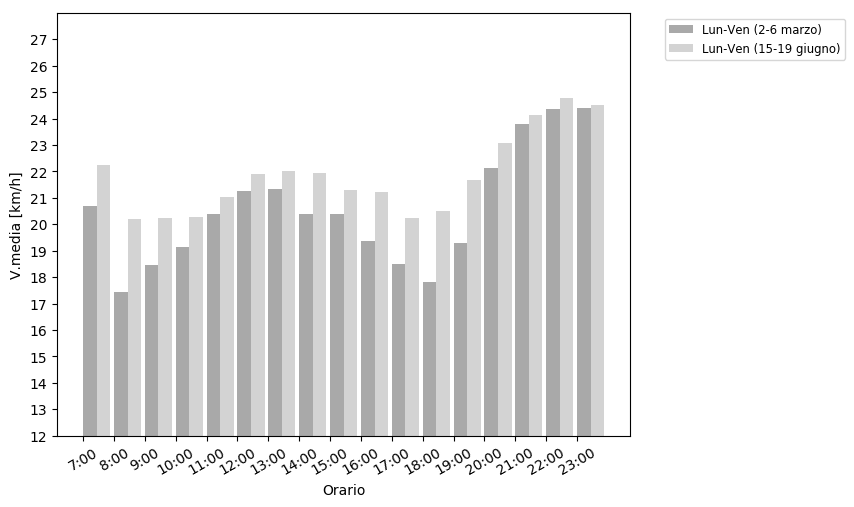
\includegraphics[scale=0.8]{vmedia_oraria_auto_prepostlock_week}
	\caption{Velocità media in auto [km/h] di ora in ora pre e post lockdown. I valori sull'asse delle ordinate variano tra 12 e 27.}
	\label{image:22}
\end{figure}

\begin{figure}[H]
	\centering
	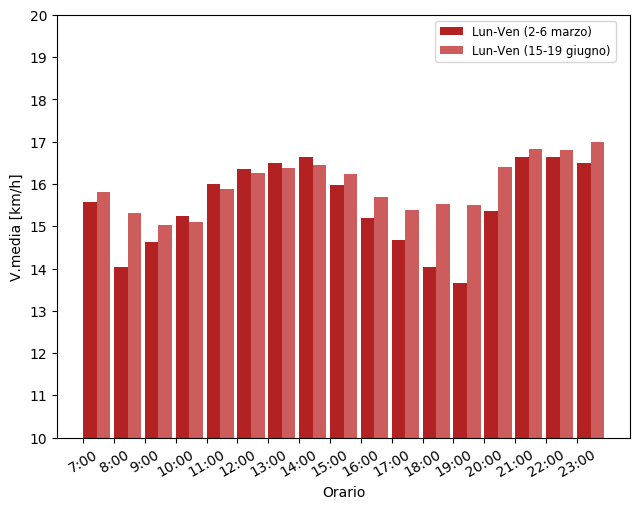
\includegraphics[scale=0.8]{vmedia_oraria_enjoy_prepostlock_week}
	\caption{Velocità media in Enjoy [km/h] di ora in ora pre e post lockdown. I valori sull'asse delle ordinate variano tra 10 e 20.}
	\label{image:24}
\end{figure}














\chapter{Conclusioni}
\section{Riflessione sul risultato}

Il risultato ottenuto dal confronto tra bicicletta e servizio di car sharing Enjoy sulla base dell'orario risulta molto interessante sotto diversi aspetti. Il primo è sicuramente la somiglianza del grafico stesso, \ref{image:12}, con quello delle prestazioni del car sharing nel grafico \ref{image:4}, che cattura la grande influenza della congestione stradale sull'efficienza in termini di tempo dell'uso dell'auto, sia essa di proprietà o condivisa. L'influenza del traffico sul servizio di car sharing preso in considerazione ha fatto sì che nelle ore intorno alle 8:00 e ancora intorno alle 18:00, lo stesso percorso è stato coperto in bicicletta nello stesso tempo se non più velocemente il 45\% delle volte, quasi 1 volta su 2. A giudicare da questo risultato, seppur prodotto sinteticamente, sembra che il servizio di car sharing riesca nell'intento di risolvere i primi due problemi principali dell'automobile, citati precedentemente, ovvero l'inquinamento, usando flotte di veicoli in linea con l'ultimo standard di emissioni euro e talvolta impiegando anche veicoli totalmente elettrici, e il costo, abbattuto dalla "condivisione" del mezzo, e quindi riducendo il pagamento al solo tempo di utilizzo. Ovviamente, il terzo problema riguardo l'efficienza rimane, risultando anche più pesante visto il tempo medio di 6 minuti per raggiungere la prima auto libera più vicina.

All'atto pratico però non risulta fattibile sostituire il servizio di car sharing o dei mezzi pubblici per fare così tanti chilometri pedalando, dato che si tratta di un'attività fisica medio-intensa e che può risultare stancante se fatta per più di 20 minuti. Tuttavia, per effettuare questo studio non si è preso in considerazione uno dei mezzi alternativi in gran diffusione nelle più grandi città del mondo, diretto concorrente della bicicletta e delle sue varianti a pedalata assistita: il monopattino elettrico.
Il monopattino elettrico infatti ha una velocità massima di 25 km/h, contro i 15 km/h di una pedalata normale in bicicletta, e può essere comprato per un costo che va dai 500 euro in sù oppure noleggiato (in mobilità condivisa) da uno dei tanti provider come Helbiz per €0.25 al minuto. Risulta molto più pratico da distribuire nella città e difatti sono molto diffusi, con un tempo medio per trovarne uno inferiore a quello del car sharing. Visti i suoi pregi e la sua velocità più alta rispetto alla bici, non sarebbe improbabile che tale mezzo riesca a battere il car sharing negli orari di punta più del 50\% delle volte e aumentando la percentuale anche nelle ore con meno traffico. Va inoltre fatta una nota riguardo l'economicità in caso di utilizzo di tale mezzo in mobilità condivisa: nel car sharing, si è presa in considerazione la lista delle auto libere solo ed esclusivamente di un servizio, Enjoy, di fatto aumentando il tempo di ricerca di un auto in mobilità condivisa in generale, per via di una quota fissa da pagare annualmente a ciascuno dei provider che si intende utilizzare, il che sposta la scelta del servizio al momento dell'iscrizione che per la maggior parte dei casi ricade su un unico provider. Al contrario, per i servizi sharing del monopattino non è richiesta nessuna documentazione ne quota fissa da pagare annualmente, ma si paga solo l'utilizzo.

\section{Possibili estensioni}

\chapter{Ringraziamenti}
e

\bibliographystyle{plain}
\bibliography{Biblio}
\end{document}
